\chapter{Evaluation}
\label{ch5}


\section{Sliding Window - HDNN - MLP}
Chen et.al. \cite{b8} has used sliding window technique with to localize the object (vehicle) in the input image. Fetaure extraction from each localized window is done using hybrid deep convolutional neural network (HDNN). Finally, classification of the extracted feature has been done using multi-layer perceptron (MLP). 

\subsection{Dataset Description}
The authors have collected 63 images of San Francisco city, having resolution $1368\times 972$ from Google earth. Out of these, 31 images are used for training, in which there were 3901 vehicles present. And rest of the 32 images were used for testing, in which 2870 vehicles were present. 
\subsection{Results}
Accuracy metrics used here are: 

\begin{figure}[!htbp]
\centerline{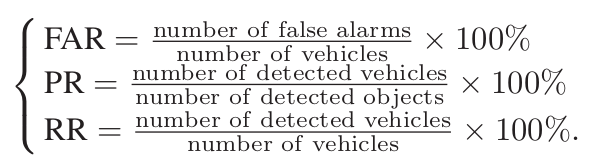
\includegraphics[height=25mm,width=90mm]{img/fig15.png}}
\caption{FAR=False Alarm Rate, PR=Precision Rate, RR=Recall Rate. Source: \cite{b8}}
\label{fig15}
\end{figure}

The authors have experimented with the blocks of different feature scale in HDNN and they have found out that an architecture of blocks with feature scale 44-20-20 works the best with 95\% recall and only 12.8\% false alarm rate. Here, 44 means that the first block has feature scale $44\times 44$, similar for 20 also. The results are shown in figure \ref{fig16}. They have also compared the precision and recall rate of differently architectured HDNN and traditional deep convolutional neural network (DNN). The results of the comparison of precision and recall rate is given in the figure \ref{fig17}.  

\begin{figure}[!htbp]
\centerline{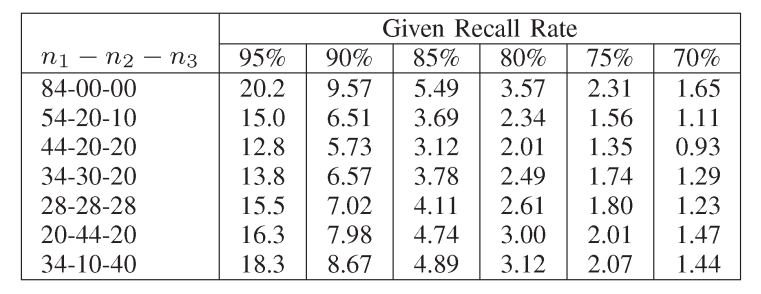
\includegraphics[height=30mm,width=90mm]{img/fig16.png}}
\caption{Relation between architecture of HDNN and FAR. Source: \cite{b8}}
\label{fig16}
\end{figure}

\begin{figure}[!htbp]
\centerline{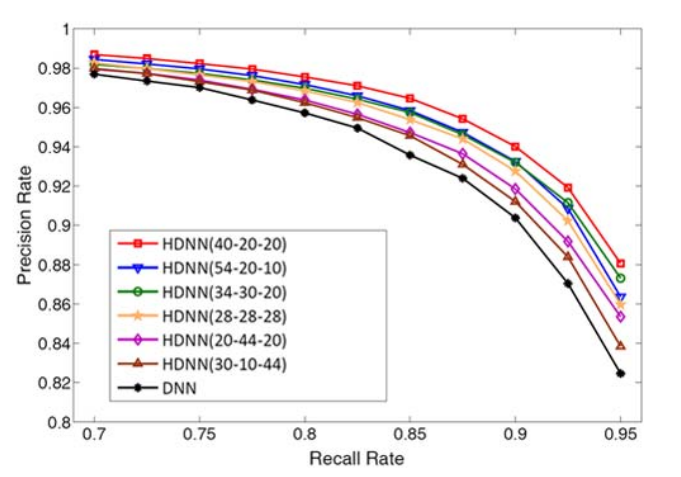
\includegraphics[height=60mm,width=80mm]{img/fig17.png}}
\caption{``Recall precision curves of HDNNs and DNN". Source: \cite{b8}}
\label{fig17}
\end{figure}


\section{ELSD - CNN and HOG - SVM}

\subsection{Dataset Description}
The authors have collected 54 images from Google Earth. 42 images has been used for training and parameter selection in ELSD while other images were used for testing purposes. By applying ELSD on 42 training samples, they have got 4264 positive samples and 7119 negative samples. They have also done data augmentation by rotating the images in every \ang{45} for more generality. After data augmentation, the number of positive and negative samples were 34112 and 56952 respectively. The test dataset contains 12 images of size $3712\times 3008$ pixels.

\subsection{Results}
Zhang et.al.\cite{b6} has used ellipse and line segment detector (ELSD) for candidate selection, CNN and HOG for feature extraction and linear SVM for classification. 
\par The authors have experimented with different values of circle threshold $\eta$ in their modified ELSD method. The results are given below: 

\begin{figure}[!htbp]
\centerline{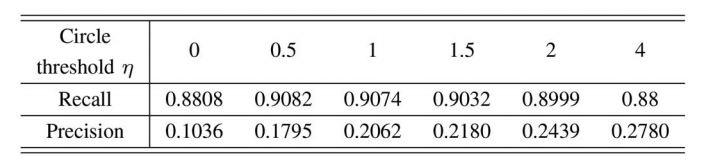
\includegraphics[height=20mm,width=90mm]{img/fig18.png}}
\caption{Precision and recall for certain values of $\eta$. Source: \cite{b6}}
\label{fig18}
\end{figure}

The modified ELSD method has achieved \textbf{90.74\%} recall rate with \textbf{26.12\%} precision rate. And linear SVM with HOG-CNN as feature vector has achieved \textbf{91.84\%} recall rate and \textbf{97.51\%} precision rate. The result of applying HOG-CNN on test images is depicted in the figure \ref{fig19}

\begin{figure}[!htbp]
\centerline{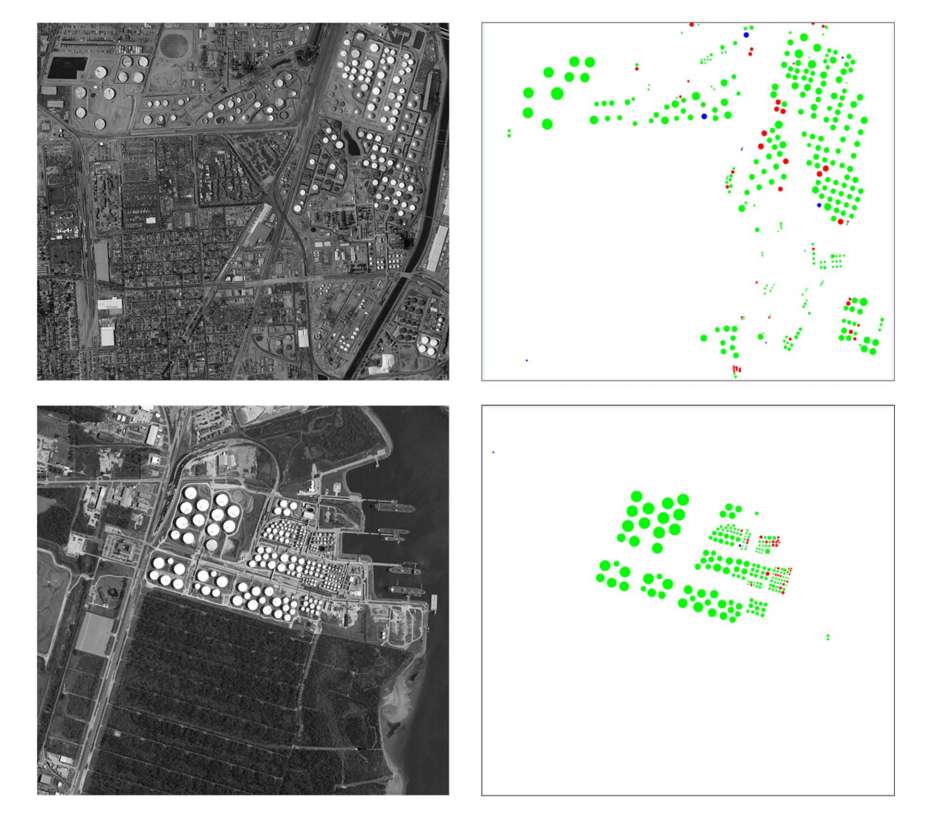
\includegraphics[height=130mm,width=150mm]{img/fig19.png}}
\caption{Examples of applying HOG-CNN. Source: \cite{b6}}
\label{fig19}
\end{figure}



\section{BING - CNN - MLP}
In this paper \cite{b5}, the authors has used binarized normed gradients for object localization, CNN for feature extraction and MLP for classification. 
\subsection{Dataset Description}
The authors have collected 500 positive image patches of aircraft and 5000 negative image patches from Google Earth. Then the 500 positive image patches were augmented by rotation of \ang{90} for 4 times, which resulted into 2000 image patches. 
\par The test dataset has 26 images of varying sizes of $565\times 369$ to $1484\times 865$.

\subsection{Results}
Here also the false alarm rate, precision rate and recall rate has been used as accuracy metrics. They are described in the figure \ref{fig15}. 
\par The authors have achieved \textbf{90.05\%} of precision rate with \textbf{80\%} of recall rate. And also the false alarm rate is \textbf{17.66\%} with \textbf{85\%} of recall rate. The variation of false alarm rate with recall rate is given below:\\ \\
\begin{tabu} to 0.9\textwidth { | X[l] | X[c] | }
 \hline
 \textbf{False Alarm Rate} & \textbf{Recall Rate} \\
 \hline
 3.75\%  & 65\%\\
\hline
4.42\% & 70\%\\
\hline
7.28\% & 75\%\\
\hline
9.27\% & 80\%\\
\hline
17.66\% & 85\%\\
\hline
\end{tabu}
\\ \\
The results of applying BING-CNN on test images is depicted in figure \ref{fig20}.

\begin{figure}[!htbp]
\centerline{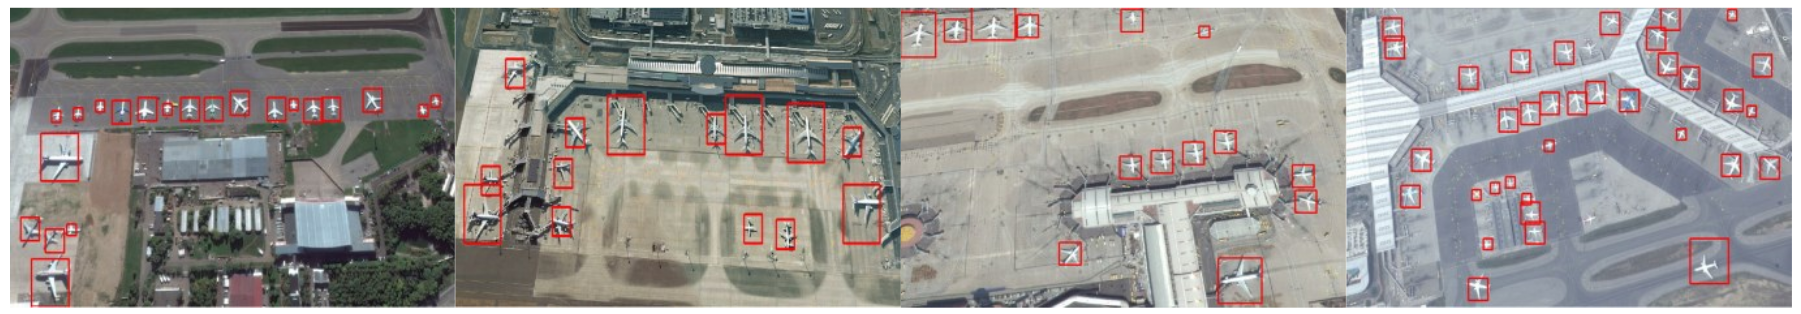
\includegraphics[height=50mm,width=160mm]{img/fig20.png}}
\caption{Examples of applying BING-CNN. Source: \cite{b5}}
\label{fig20}
\end{figure}

\par Wu .et.al.\cite{b5} have not evaluated the performance of BING on their dataset. So, the performance of BING \cite{b2} in VOC2007 test set has been described. This dataset contains 4952 images with bounding box annotations. There are 20 different classes present in the dataset. BING has achieved \textbf{99.5\%} detection rate with 5000 object proposals. Detection rate can be defined as the number of objects that are correctly detected, divided by total number of objects.


